




\section*{ID: cf0ae57a}
Distance and Density of Planetoids in the Inner Solar System\\
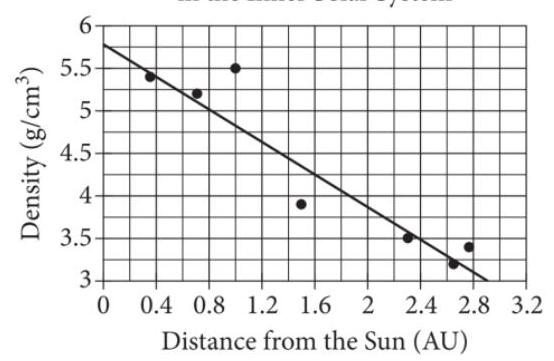
\includegraphics[max width=\textwidth, center]{2025_06_15_c6d1fe032100fbb48447g-01}

The scatterplot above shows the densities of 7 planetoids, in grams per cubic centimeter, with respect to their average distances from the Sun in astronomical units (AU). The line of best fit is also shown. An astronomer has discovered a new planetoid about 1.2 AU from the Sun. According to the line of best fit, which of the following best approximates the density of the planetoid, in grams per cubic centimeter?\\
A. 3.6\\
B. 4.1\\
C. 4.6\\
D. 5.5

\section*{ID: 58171b5e}
Each year, the value of an investment increases by $0.49 \%$ of its value the previous year. Which of the following functions best models how the value of the investment changes over time?\\
A. Decreasing exponential\\
B. Decreasing linear\\
C. Increasing exponential\\
D. Increasing linear

The scatterplot shows the relationship between $x$ and $y$. A line of best fit is also shown.\\
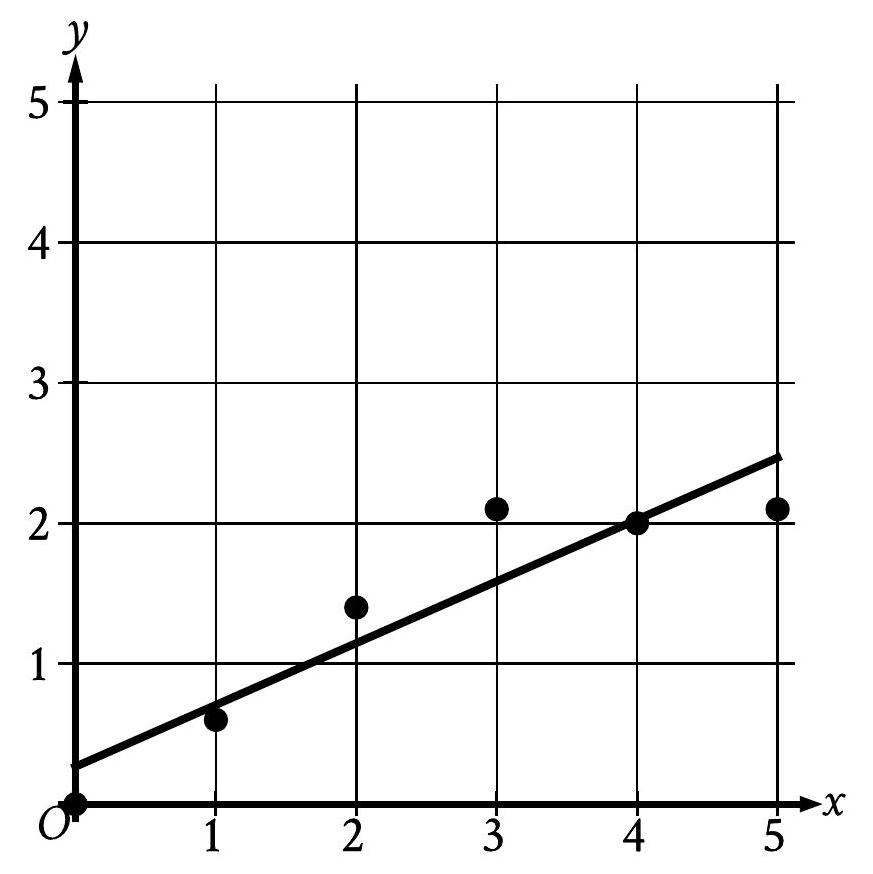
\includegraphics[max width=\textwidth, center]{2025_06_15_c6d1fe032100fbb48447g-03}

Which of the following is closest to the slope of the line of best fit shown?\\
A. -2.27\\
B. -0.44\\
C. 0.44\\
D. 2.27\\
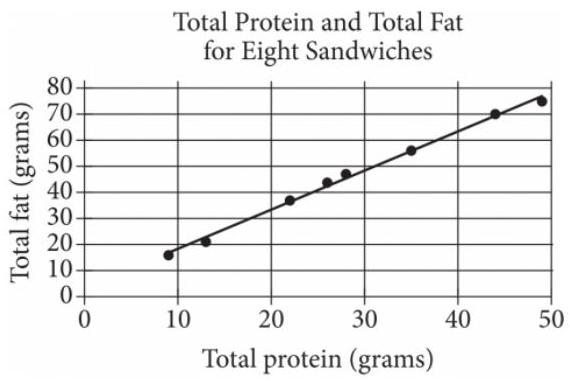
\includegraphics[max width=\textwidth, center]{2025_06_15_c6d1fe032100fbb48447g-04}

The scatterplot above shows the numbers of grams of both total protein and total fat for eight sandwiches on a restaurant menu. The line of best fit for the data is also shown. According to the line of best fit, which of the following is closest to the predicted increase in total fat, in grams, for every increase of 1 gram in total protein?\\
A. 2.5\\
B. 2.0\\
C. 1.5\\
D. 1.0

\section*{ID: 50b2807e}
The scatterplot shows the relationship between two variables, $x$ and $y$.\\
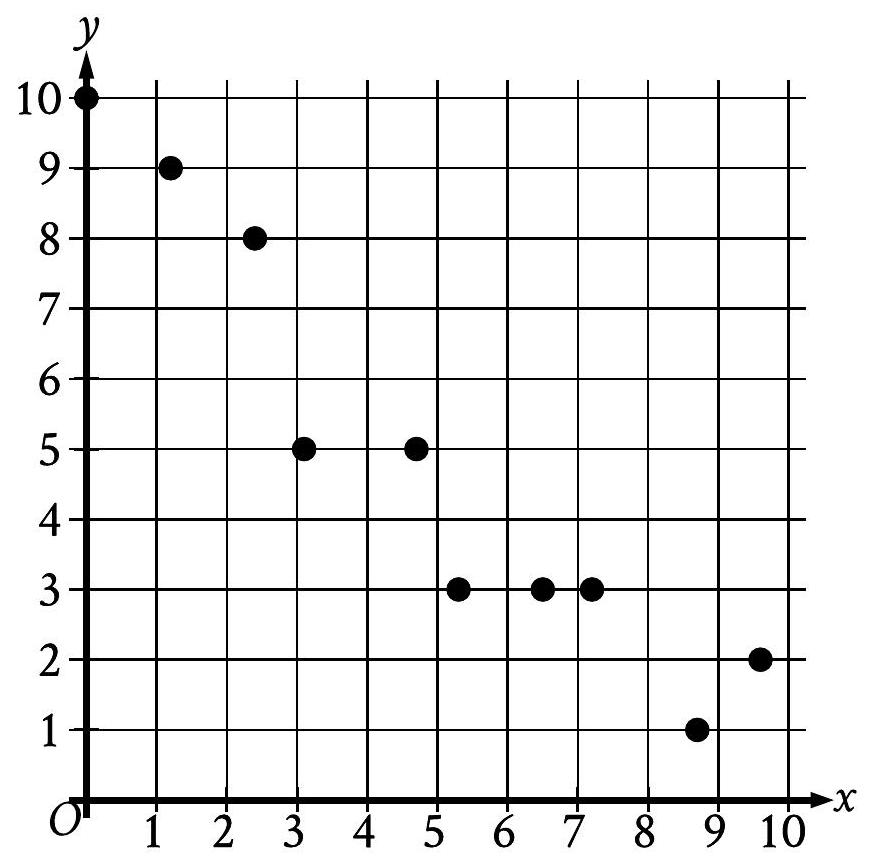
\includegraphics[max width=\textwidth, center]{2025_06_15_c6d1fe032100fbb48447g-05}

Which of the following equations is the most appropriate linear model for the data shown?\\
A. $y=0.9+9.4 x$\\
B. $y=0.9-9.4 x$\\
C. $y=9.4+0.9 x$\\
D. $y=9.4-0.9 x$

\section*{ID: af142f8d}
\begin{center}
\begin{tabular}{|c|c|c|}
\hline
 & Amount invested & Balance increase \\
\hline
Account A & $\$ 500$ & $6 \%$ annual interest \\
\hline
Account B & $\$ 1,000$ & $\$ 25$ per year \\
\hline
\end{tabular}
\end{center}

Two investments were made as shown in the table above. The interest in Account A is compounded once per year. Which of the following is true about the investments?\\
A. Account A always earns more money per year than Account B.\\
B. Account A always earns less money per year than Account B.\\
C. Account A earns more money per year than Account B at first but eventually earns less money per year.\\
D. Account A earns less money per year than Account B at first but eventually earns more money per year.

\section*{ID: 9b5b23fc}
For $x>0$, the function $f$ is defined as follows:

$$
f(x) \text { equals } 201 \% \text { of } x
$$

Which of the following could describe this function?\\
A. Decreasing exponential\\
B. Decreasing linear\\
C. Increasing exponential\\
D. Increasing linear

\section*{ID: fdfc90e4}
The scatterplot shows the relationship between two variables, $x$ and $y$. A line of best fit for the data is also shown.\\
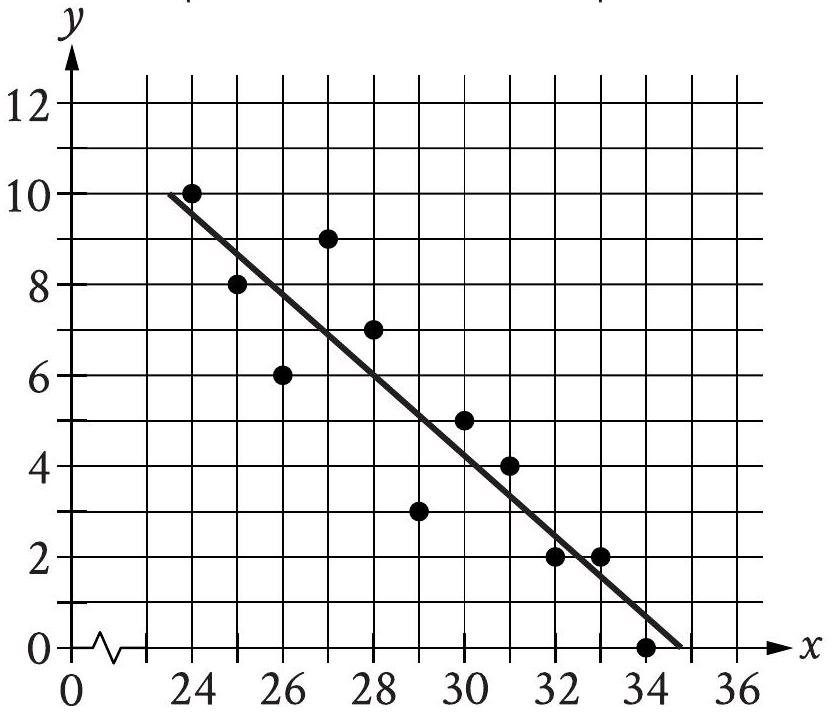
\includegraphics[max width=\textwidth, center]{2025_06_15_c6d1fe032100fbb48447g-08}

At $x=32$, which of the following is closest to the $y$-value predicted by the line of best fit?\\
A. 0.4\\
B. 1.5\\
C. 2.4\\
D. 3.3

\section*{ID: 79137c1b}
\begin{center}
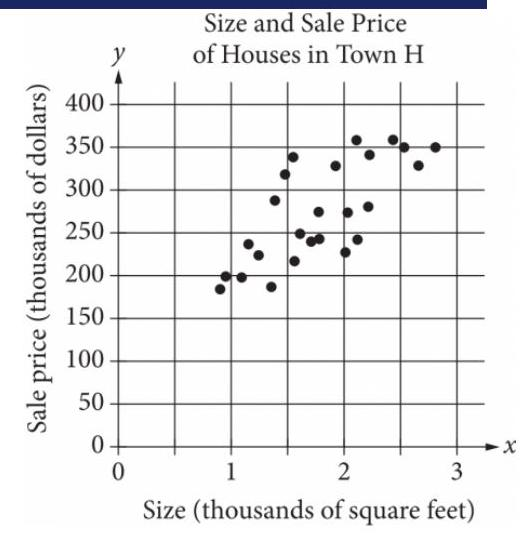
\includegraphics[max width=\textwidth]{2025_06_15_c6d1fe032100fbb48447g-09}
\end{center}

The scatterplot above shows the size $x$ and the sale price $y$ of 25 houses for sale in Town H . Which of the following could be an equation for a line of best fit for the data?\\
A. $y=200 x+100$\\
B. $y=100 x+100$\\
C. $y=50 x+100$\\
D. $y=100 x$\\
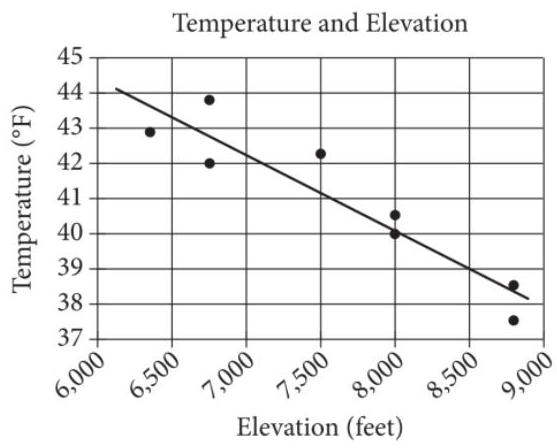
\includegraphics[max width=\textwidth, center]{2025_06_15_c6d1fe032100fbb48447g-10}

The scatterplot above shows the high temperature on a certain day and the elevation of 8 different locations in the Lake Tahoe Basin. A line of best fit for the data is also shown. Which of the following statements best describes the association between the elevation and the temperature of locations in the Lake Tahoe Basin?\\
A. As the elevation increases, the temperature tends to increase.\\
B. As the elevation increases, the temperature tends to decrease.\\
C. As the elevation decreases, the temperature tends to decrease.\\
D. There is no association between the elevation and the temperature.\\





























































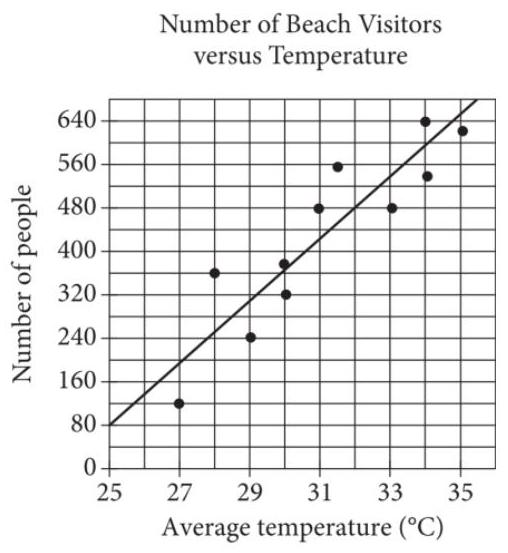
\includegraphics[max width=\textwidth, center]{2025_06_15_c6d1fe032100fbb48447g-21}

Each dot in the scatterplot above represents the temperature and the number of people who visited a beach in Lagos, Nigeria, on one of eleven different days. The line of best fit for the data is also shown. The line of best fit for the data has a slope of approximately 57. According to this estimate, how many additional people per day are predicted to visit the beach for each $5^{\circ} \mathrm{C}$ increase in average temperature?

An airplane descends from an altitude of 9,500 feet to 5,000 feet at a constant rate of 400 feet per minute. What type of function best models the relationship between the descending airplane's altitude and time?\\
A. Decreasing exponential\\
B. Decreasing linear\\
C. Increasing exponential\\
D. Increasing linear

\section*{ID: 3c5b19ef}
\begin{center}
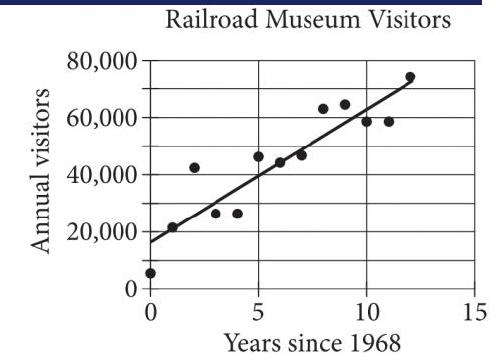
\includegraphics[max width=\textwidth]{2025_06_15_c6d1fe032100fbb48447g-23}
\end{center}

The scatterplot above shows the number of visitors to a railroad museum in Pennsylvania each year from 1968 to 1980, where $t$ is the number of years since 1968 and $n$ is the number of visitors. A line of best fit is also shown. Which of the following could be an equation of the line of best fit shown?\\
A. $n=16,090+4,680 t$\\
B. $n=4,690+16,090 t$\\
C. $n=16,090+9,060 t$\\
D. $n=9,060+16,090 t$

The scatterplot shows the relationship between the length of time $y$, in hours, a certain bird spent in flight and the number of days after January $11, x$.\\
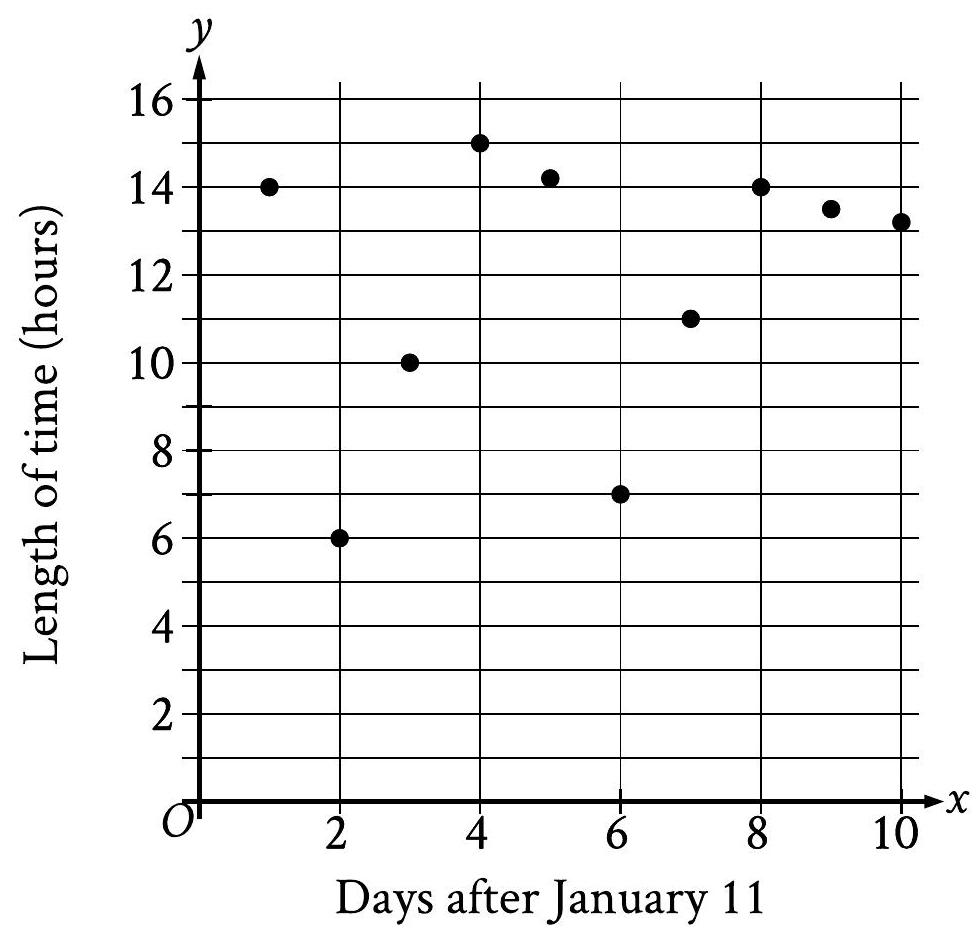
\includegraphics[max width=\textwidth, center]{2025_06_15_c6d1fe032100fbb48447g-24}

What is the average rate of change, in hours per day, of the length of time the bird spent in flight on January 13 to the length of time the bird spent in flight on January 15 ?

\section*{ID: a6b2fcce}
\begin{center}
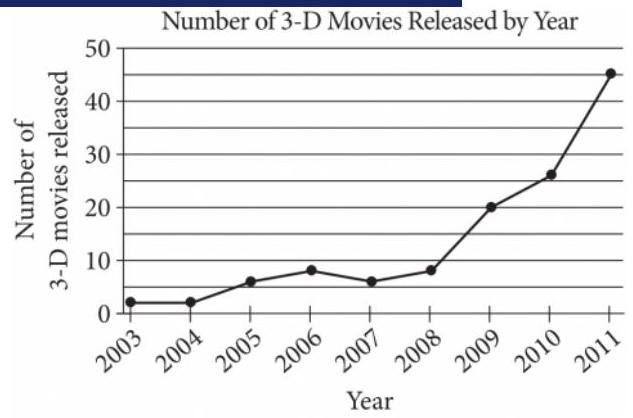
\includegraphics[max width=\textwidth]{2025_06_15_c6d1fe032100fbb48447g-25}
\end{center}

According to the line graph above, between which two consecutive years was there the greatest change in the number of 3-D movies released?\\
A. 2003-2004\\
B. 2008-2009\\
C. 2009-2010\\
D. 2010-2011

\section*{ID: c9dd92b1}
\begin{center}
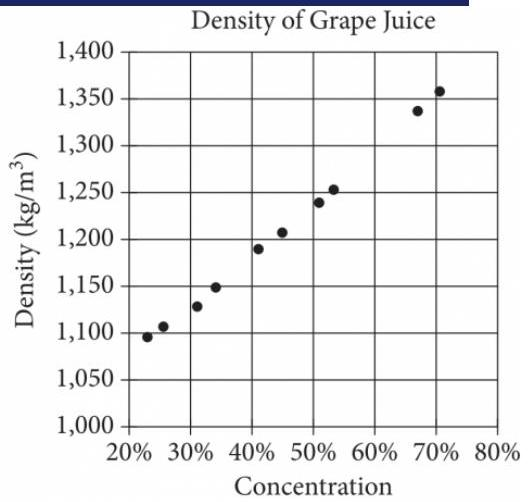
\includegraphics[max width=\textwidth]{2025_06_15_c6d1fe032100fbb48447g-26}
\end{center}

The densities of different concentrations of grape juice are shown in the scatterplot above. According to the trend shown by the data, which of the following is closest to the predicted density, in kilograms per cubic meter ( $\mathrm{kg} / \mathrm{m}^{3}$ ), for grape juice with a concentration of 60\%?\\
A. 1,200\\
B. 1,250\\
C. 1,300\\
D. 1,350\\
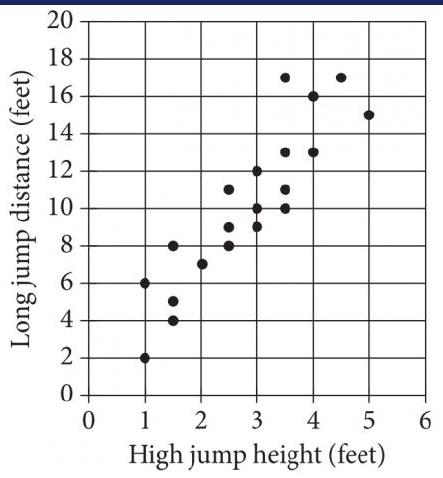
\includegraphics[max width=\textwidth, center]{2025_06_15_c6d1fe032100fbb48447g-27}

Each dot in the scatterplot above represents the height $x$, in feet, in the high jump, and the distance $y$, in feet, in the long jump, made by each student in a group of twenty students. The graph of which of the following equations is a line that most closely fits the data?\\
A. $y=0.82 x+3.30$\\
B. $y=0.82 x-0.82$\\
C. $y=3.30 x+0.82$\\
D. $y=3.30 x-3.30$

\section*{ID: 1e1027a7}
\begin{center}
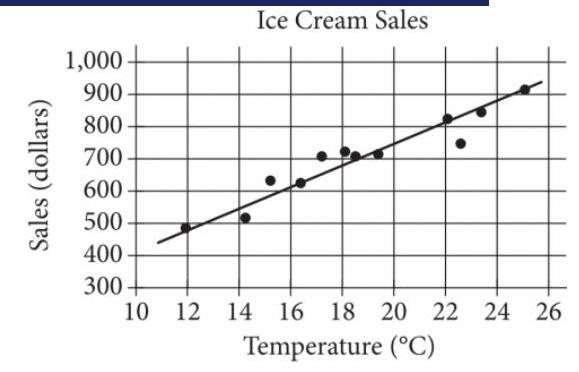
\includegraphics[max width=\textwidth]{2025_06_15_c6d1fe032100fbb48447g-28}
\end{center}

The scatterplot above shows a company's ice cream sales $d$, in dollars, and the high temperature $t$, in degrees Celsius $\left({ }^{\circ} \mathrm{C}\right)$, on 12 different days. A line of best fit for the data is also shown. Which of the following could be an equation of the line of best fit?\\
A. $d=0.03 t+402$\\
B. $d=10 t+402$\\
C. $d=33 t+300$\\
D. $d=33 t+84$

\section*{ID: 7fd284ac}
Income and Percent of Total Expenses Spent\\
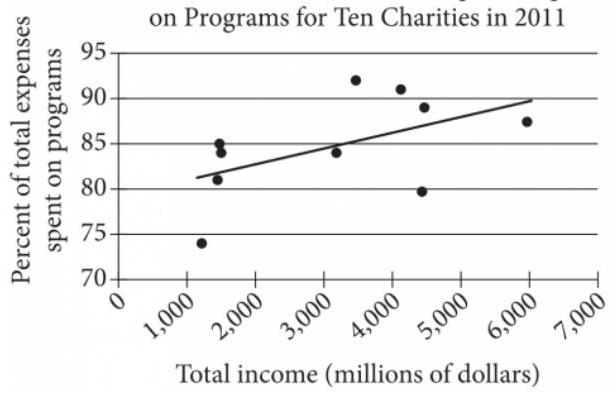
\includegraphics[max width=\textwidth, center]{2025_06_15_c6d1fe032100fbb48447g-29}

The scatterplot above shows data for ten charities along with the line of best fit. For the charity with the greatest percent of total expenses spent on programs, which of the following is closest to the difference of the actual percent and the percent predicted by the line of best fit?\\
A. $10 \%$\\
B. $7 \%$\\
C. $4 \%$\\
D. $1 \%$

The scatterplot shows the relationship between two variables, $x$ and $y$. A line of best fit is also shown.\\
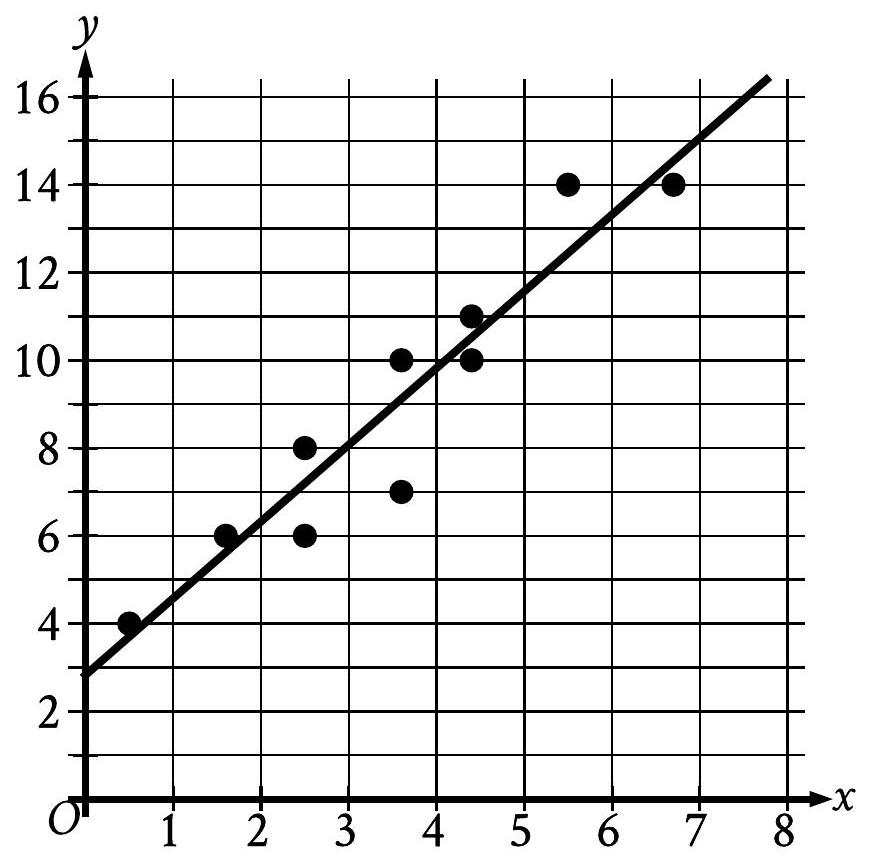
\includegraphics[max width=\textwidth, center]{2025_06_15_c6d1fe032100fbb48447g-30}

Which of the following equations best represents the line of best fit shown?\\
A. $y=2.8+1.7 x$\\
B. $y=2.8-1.7 x$\\
C. $y=-2.8+1.7 x$\\
D. $y=-2.8-1.7 x$

\section*{ID: 7ac5d686}
An inspector begins a day of work with a large sample of shirts that need to be checked for defects. The inspector works at a constant rate throughout the morning. What type of model is best to model the number of shirts remaining to be checked for defects at any given time throughout the morning?\\
A. A linear model with a positive slope\\
B. A linear model with a negative slope\\
C. An exponential growth model\\
D. An exponential decay model

\section*{ID: f46139df}
The scatterplot shows the relationship between two variables, $x$ and $y$. A line of best fit for the data is also shown.\\
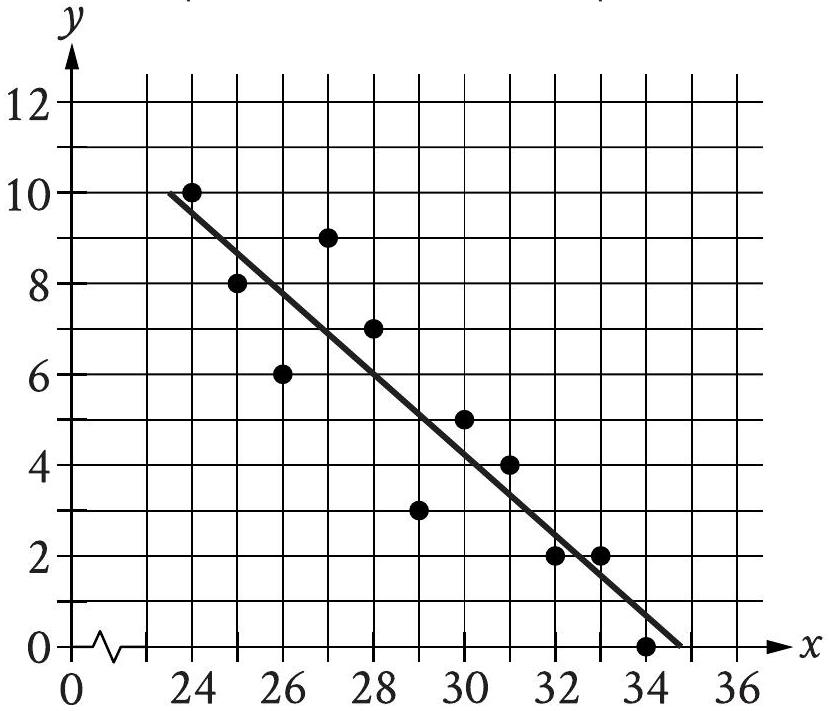
\includegraphics[max width=\textwidth, center]{2025_06_15_c6d1fe032100fbb48447g-32}

At $x=25.5$, which of the following is closest to the $y$-value predicted by the line of best fit?\\
A. 6.2\\
B. 7.3\\
C. 8.2\\
D. 9.1

\section*{ID: 9d88a3e3}
\begin{center}
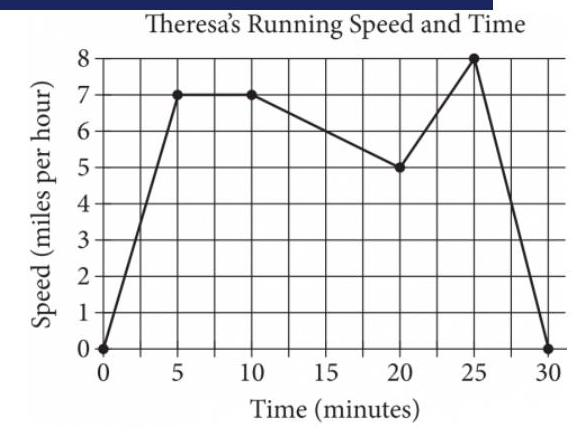
\includegraphics[max width=\textwidth]{2025_06_15_c6d1fe032100fbb48447g-33}
\end{center}

Theresa ran on a treadmill for thirty minutes, and her time and speed are shown on the graph above. According to the graph, which of the following statements is NOT true concerning Theresa's run?\\
A. Theresa ran at a constant speed for five minutes.\\
B. Theresa's speed was increasing for a longer period of time than it was decreasing.\\
C. Theresa's speed decreased at a constant rate during the last five minutes.\\
D. Theresa's speed reached its maximum during the last ten minutes.\\
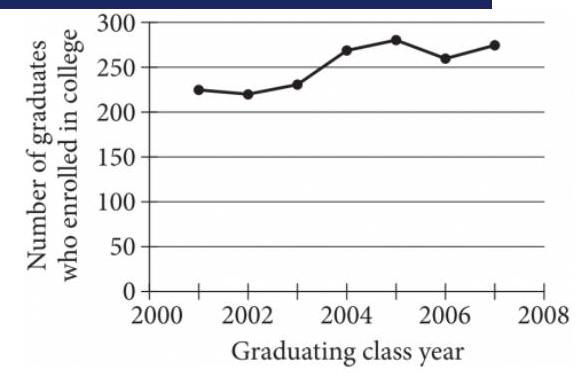
\includegraphics[max width=\textwidth, center]{2025_06_15_c6d1fe032100fbb48447g-34}

The line graph shows the number of graduates from the classes of 2001 through 2007 at a certain school who enrolled in college within 24 months of graduation. Of the following, which class had the fewest graduates who enrolled in college within 24 months of graduation?\\
A. 2002\\
B. 2004\\
C. 2005\\
D. 2007

\section*{ID: d6af3572}
\begin{center}
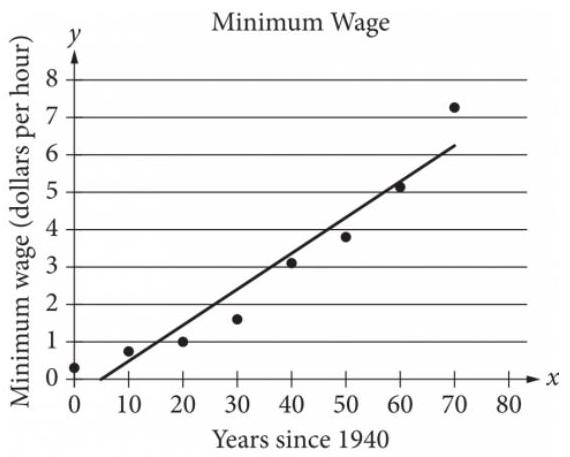
\includegraphics[max width=\textwidth]{2025_06_15_c6d1fe032100fbb48447g-35}
\end{center}

The scatterplot above shows the federal-mandated minimum wage every 10 years between 1940 and 2010. A line of best fit is shown, and its equation is $y=0.096 x-0.488$. What does the line of best fit predict about the increase in the minimum wage over the 70-year period?\\
A. Each year between 1940 and 2010, the average increase in minimum wage was 0.096 dollars.\\
B. Each year between 1940 and 2010, the average increase in minimum wage was 0.49 dollars.\\
C. Every 10 years between 1940 and 2010, the average increase in minimum wage was 0.096 dollars.\\
D. Every 10 years between 1940 and 2010, the average increase in minimum wage was 0.488 dollars.

The scatterplot shows the relationship between two variables, $x$ and $y$. A line of best fit is also shown.\\
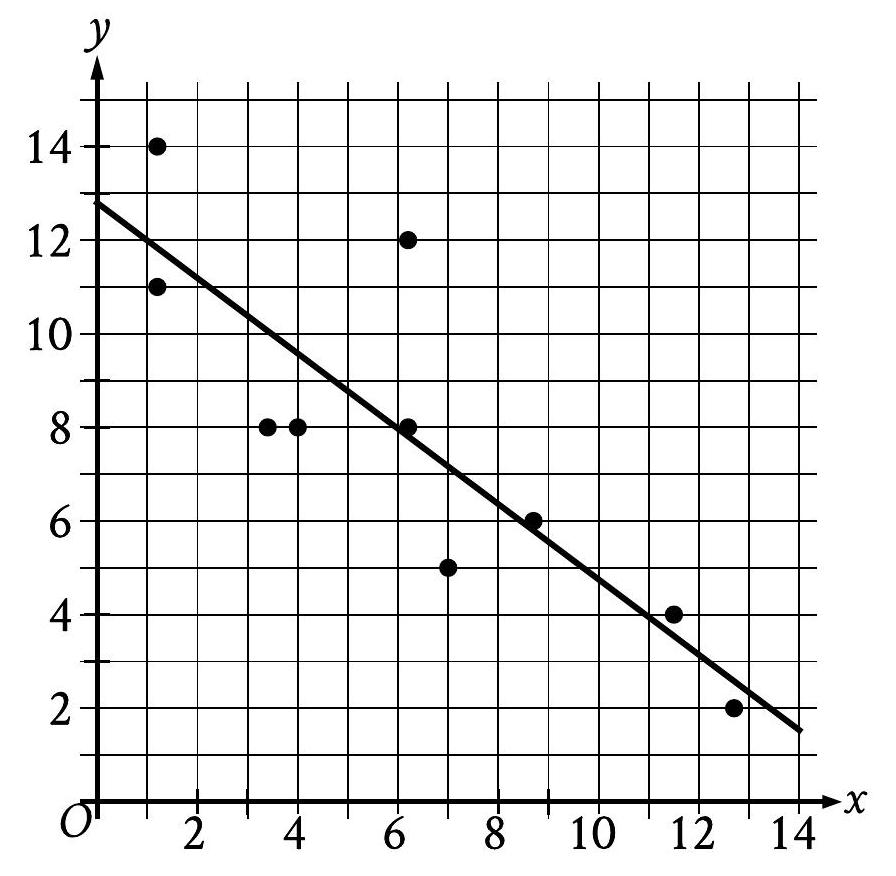
\includegraphics[max width=\textwidth, center]{2025_06_15_c6d1fe032100fbb48447g-36}

Which of the following is closest to the slope of the line of best fit shown?\\
A. -2.4\\
B. -0.8\\
C. 0.8\\
D. 2.4

\section*{ID: 9a144a01}
Which of the following is true about the values of $2^{x}$ and $2 x+2$ for $x>0$ ?\\
A. For all $x>0$, it is true that $2^{x}<2 x+2$.\\
B. For all $x>0$, it is true that $2^{x}>2 x+2$.\\
C. There is a constant $c$ such that if $0<x<c$, then $2^{x}<2 x+2$, but if $x>c$, then $2^{x}>2 x+2$.\\
D. There is a constant $c$ such that if $0<x<c$, then $2^{x}>2 x+2$, but if $x>c$, then $2^{x}<2 x+2$.

In the given scatterplot, a line of best fit for the data is shown.\\
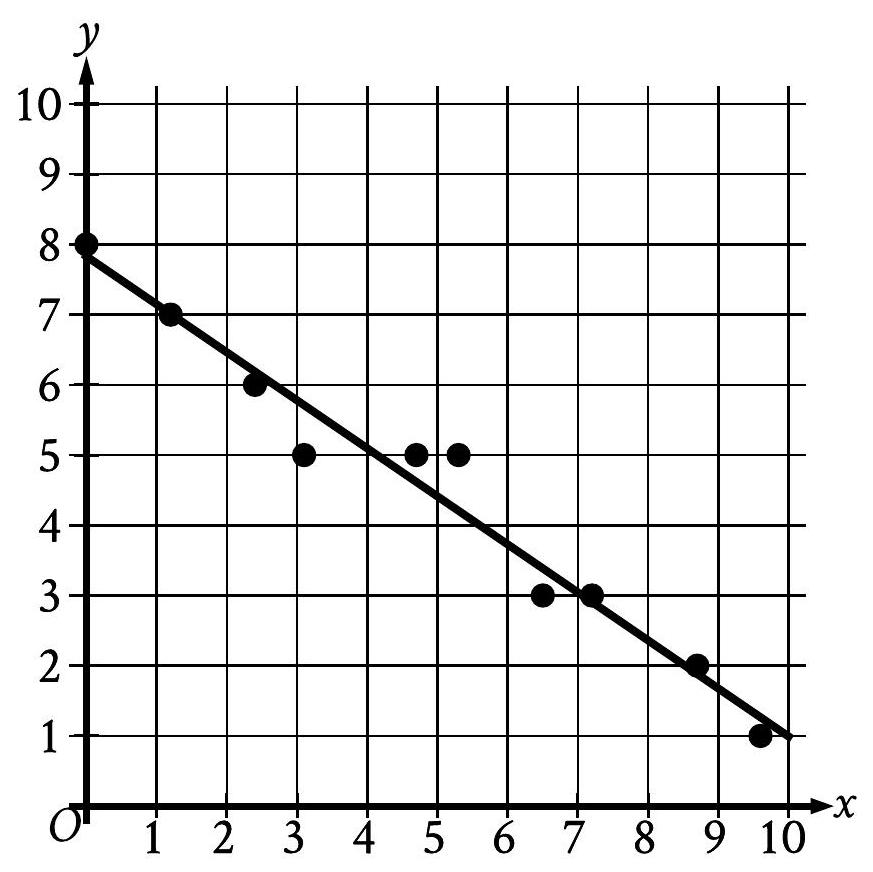
\includegraphics[max width=\textwidth, center]{2025_06_15_c6d1fe032100fbb48447g-38}

Which of the following is closest to the slope of this line of best fit?\\
A. 7\\
B. 0.7\\
C. -0.7\\
D. -7\\
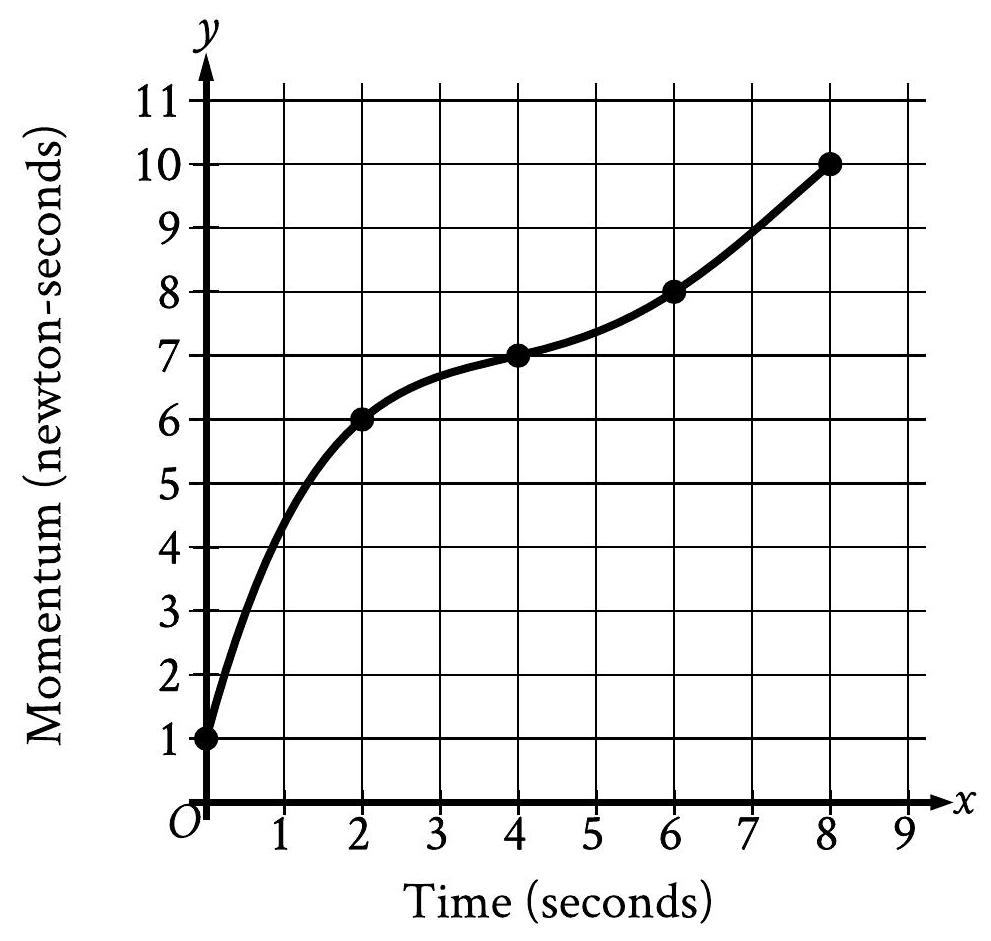
\includegraphics[max width=\textwidth, center]{2025_06_15_c6d1fe032100fbb48447g-39}

The graph shows the momentum $y$, in newton-seconds, of an object $x$ seconds after the object started moving, for $0 \leq x \leq 8$. What is the average rate of change, in newton-seconds per second, in the momentum of the object from $x=2$ to $x=6$ ?

\section*{ID: 4a2264b3}
The line graph shows the percent of cars for sale at a used car lot on a given day by model year.\\
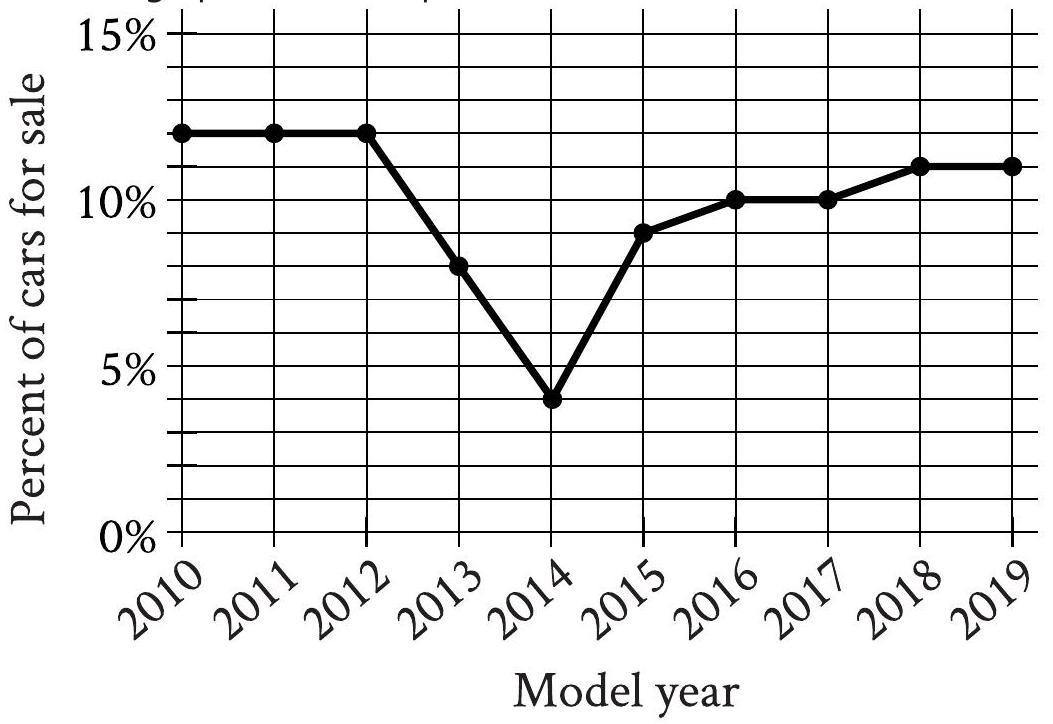
\includegraphics[max width=\textwidth, center]{2025_06_15_c6d1fe032100fbb48447g-40}

For what model year is the percent of cars for sale the smallest?\\
A. 2012\\
B. 2013\\
C. 2014\\
D. 2015\\
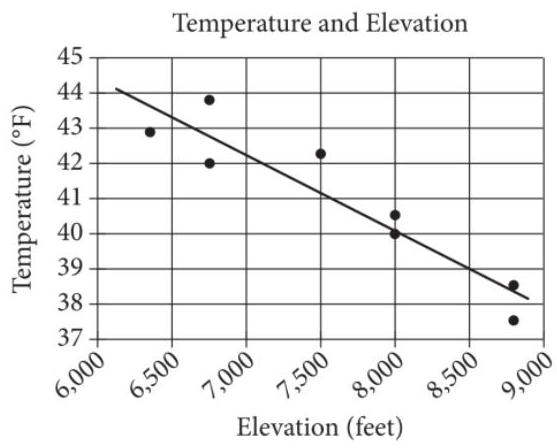
\includegraphics[max width=\textwidth, center]{2025_06_15_c6d1fe032100fbb48447g-41}

The scatterplot above shows the high temperature on a certain day and the elevation of 8 different locations in the Lake Tahoe Basin. A line of best fit for the data is also shown. What temperature is predicted by the line of best fit for a location in the Lake Tahoe Basin with an elevation of 8,500 feet?\\
A. $37^{\circ} \mathrm{F}$\\
B. $39^{\circ} \mathrm{F}$\\
C. $41^{\circ} \mathrm{F}$\\
D. $43^{\circ} \mathrm{F}$

\section*{ID: 8baf2118}
The scatterplot shows the relationship between two variables, $x$ and $y$. A line of best fit is also shown.\\
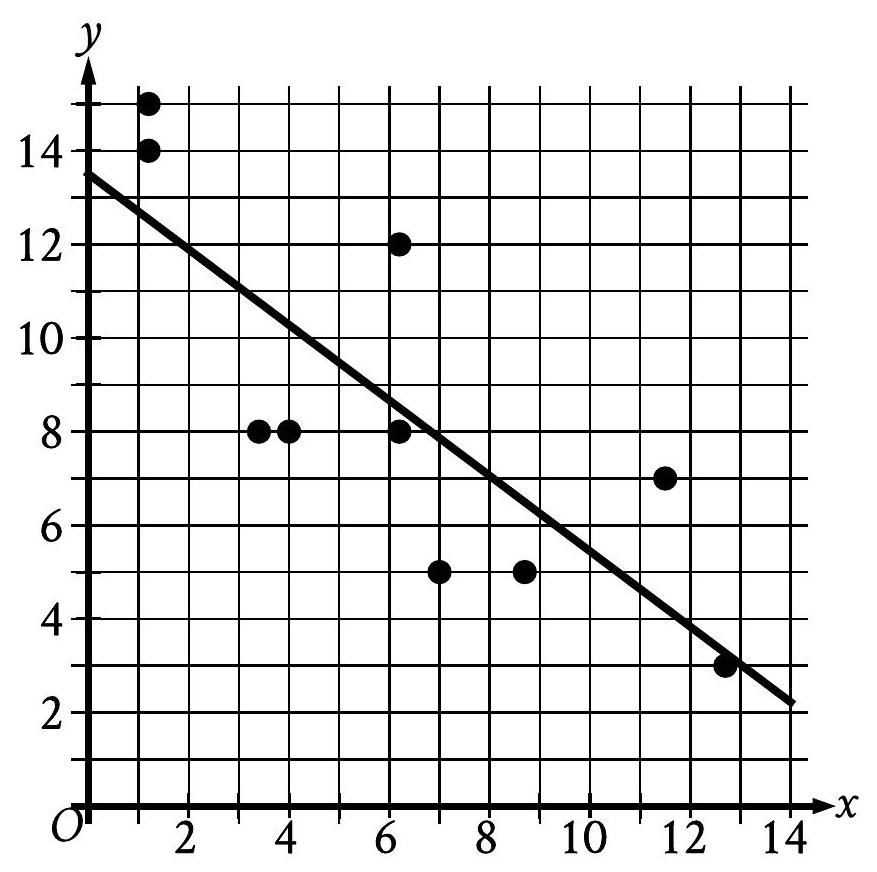
\includegraphics[max width=\textwidth, center]{2025_06_15_c6d1fe032100fbb48447g-42}

Which of the following equations best represents the line of best fit shown?\\
A. $y=13.5+0.8 x$\\
B. $y=13.5-0.8 x$\\
C. $y=-13.5+0.8 x$\\
D. $y=-13.5-0.8 x$

\section*{ID: 83272c51}
\begin{center}
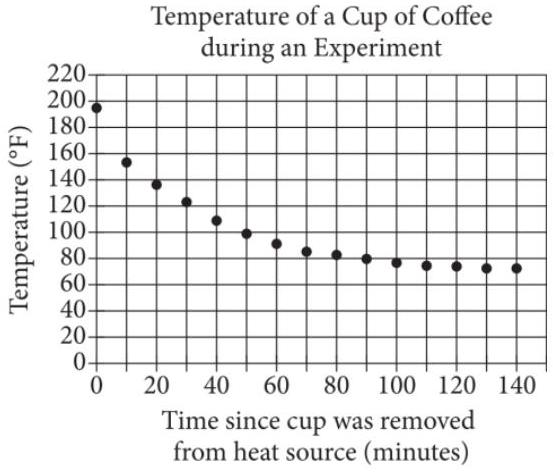
\includegraphics[max width=\textwidth]{2025_06_15_c6d1fe032100fbb48447g-43}
\end{center}

In an experiment, a heated cup of coffee is removed from a heat source, and the cup of coffee is then left in a room that is kept at a constant temperature. The graph above shows the temperature, in degrees Fahrenheit ( ${ }^{\circ} \mathrm{F}$ ), of the coffee immediately after being removed from the heat source and at 10-minute intervals thereafter. During which of the following 10-minute intervals does the temperature of the coffee decrease at the greatest average rate?\\
A. Between 0 and 10 minutes\\
B. Between 30 and 40 minutes\\
C. Between 50 and 60 minutes\\
D. Between 90 and 100 minutes

\section*{ID: 82aaa0a1}
\begin{center}
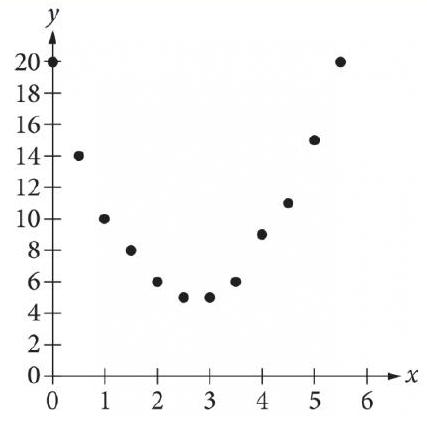
\includegraphics[max width=\textwidth]{2025_06_15_c6d1fe032100fbb48447g-44}
\end{center}

Of the following, which is the best model for the data in the scatterplot?\\
A. $y=2 x^{2}-11 x-20$\\
B. $y=2 x^{2}-11 x+20$\\
C. $y=2 x^{2}-5 x-3$\\
D. $y=2 x^{2}-5 x+3$

\section*{ID: 1adb39f0}
The scatterplot shows the relationship between two variables, $x$ and $y$. A line of best fit for the data is also shown. Which of the following is closest to the difference between the $y$-coordinate of the data point with $x=1$ and the $y$-value predicted by the line of best fit at $x=1$ ?\\
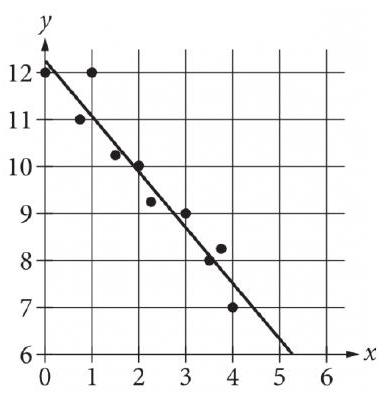
\includegraphics[max width=\textwidth, center]{2025_06_15_c6d1fe032100fbb48447g-45}\\
A. 1\\
B. 2\\
C. 5\\
D. 12


